\documentclass[12pt, a4paper, lithuanian]{article}

\usepackage[utf8x]{inputenc}

\usepackage{VUMIF}
\usepackage{listings}
\usepackage{graphicx}


% "define" Scala
\lstdefinelanguage{scala}{
  morekeywords={abstract,case,catch,class,def,%
    do,else,extends,false,final,finally,%
    for,if,implicit,import,match,mixin,%
    new,null,object,override,package,%
    private,protected,requires,return,sealed,%
    super,this,throw,trait,true,try,%
    type,val,var,while,with,yield},
  otherkeywords={=>,<-,<\%,<:,>:,\#,@},
  sensitive=true,
  morecomment=[l]{//},
  morecomment=[n]{/*}{*/},
  morestring=[b]",
  morestring=[b]',
  morestring=[b]""
}

\usepackage{color}
\definecolor{dkgreen}{rgb}{0,0.6,0}
\definecolor{gray}{rgb}{0.5,0.5,0.5}
\definecolor{mauve}{rgb}{0.58,0,0.82}


% Default settings for code listings
\lstset{frame=tb,
  language=scala,
  aboveskip=3mm,
  belowskip=3mm,
  showstringspaces=false,
  columns=flexible,
  basicstyle={\small\ttfamily},
  numbers=none,
  numberstyle=\tiny\color{gray},
  %keywordstyle=\color{blue},
  %commentstyle=\color{dkgreen},
  %stringstyle=\color{mauve},
  frame=single,
  breaklines=true,
  breakatwhitespace=true
  tabsize=3
}

% \usepackage[mathcsdepttitle]{VUMIF} % --- matematinės informatikos katedros
%     titulinio puslapio formatavimas

% Titulinio puslapio reikalai
\vumifpaper{Project report}
\title{Amsterdam Vibe}
\engtitle{Intelligent Web Applications course final project}
\author{
    \\
    Žilvinas Kučinskas \\
    Student number: 2547940 \\
    E-mail: zil.kucinskas@gmail.com
}

\supervisor{
    Mihnea Dobrescu-Balaur \\
    Student number: 2549278 \\
    E-mail: mihnea@linux.com
}
\reviewer{
  Arthur-Ervin Avramiea \\
  Student number: 2517642 \\
  E-mail: a.e.avramiea@student.vu.nl
}
\date{Amsterdam \\ 2014}

\begin{document}

\maketitle

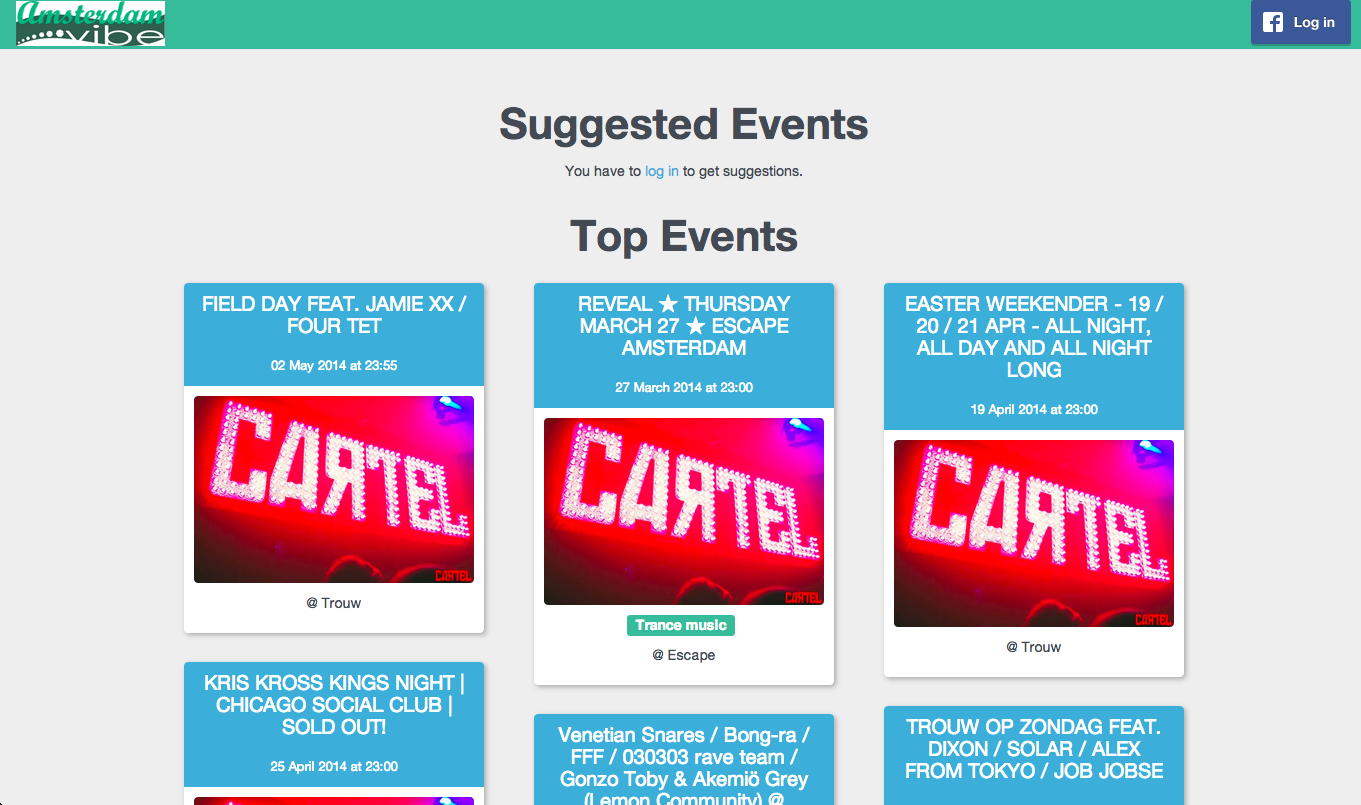
\includegraphics[width=\linewidth]{list}

\vspace{1cm}

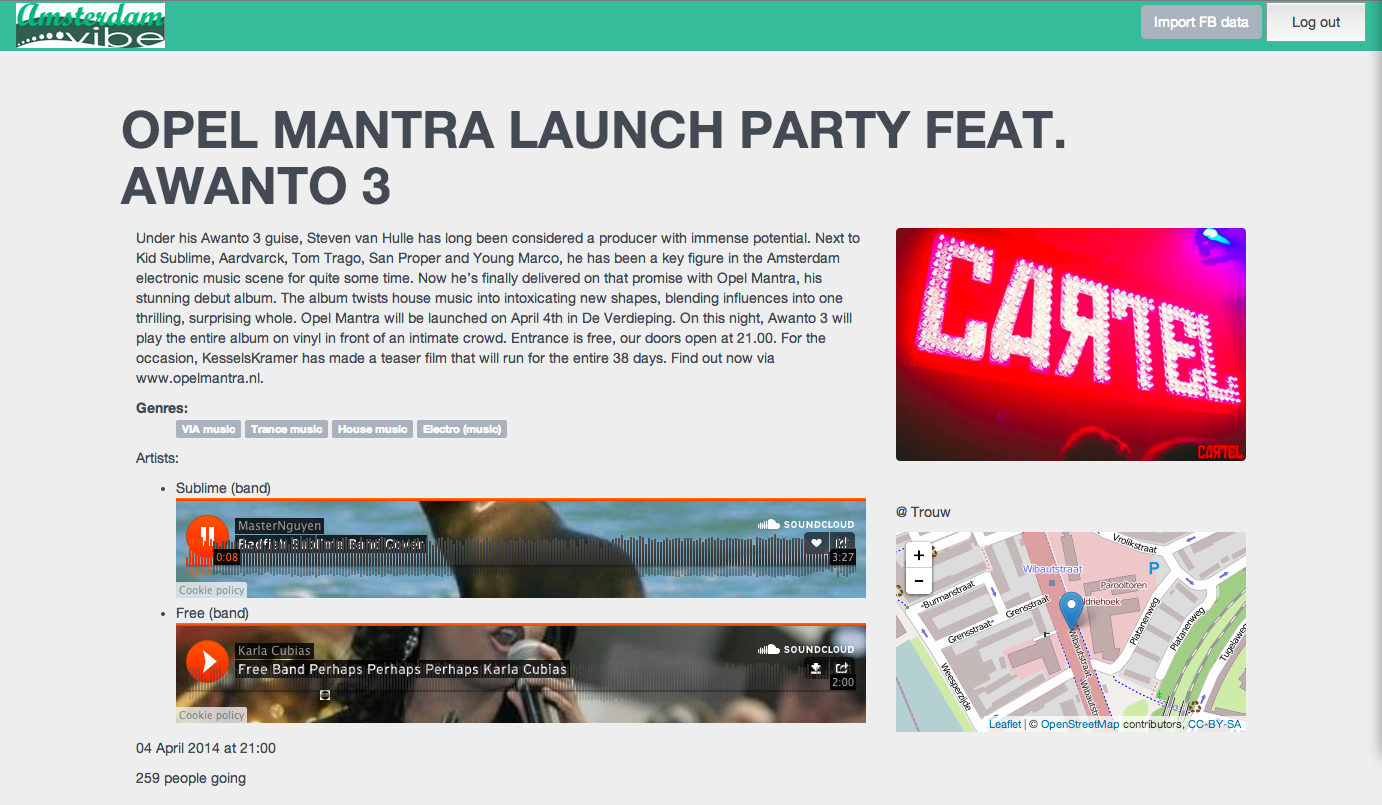
\includegraphics[width=\linewidth]{detail}

\tableofcontents

\section{Introduction}

This is a comprehensive report of the Intelligent Web Applications course final group project.

\subsection{Requirements}

There were the following requirements for the project:

\begin{itemize}
    \item Use an RDF store.

    \item Use semantic Web reasoning in your RDF store to generate new information.

    \item Integrate at least three data sources.

    \item Present the integrated information in cool, interesting and innovative ways.

    \item Interact with at least one remote SPARQL endpoint (In addition to your local RDF store).

    \item Interact with at least one non RDF Web service.

    \item Write a report about it.

\end{itemize}


\subsection{Code}

All code can be found in the following public GitHub repository:

\begin{itemize}

  \item https://github.com/TooHighToPlay/AmsterdamVibe

\end{itemize}

\subsection{Link to working application}

Working example of the application can be found on the following link:

\begin{itemize}

  \item amsterdamvibe.cloudapp.net

\end{itemize}

\section{Report}

\subsection{Idea}

  Amsterdam is famous not only for its architecture, history or beautiful sights, but also for it's vibrant nightlife. It has more than 4 million tourists coming over during the year, it also has a lot of youth people from all over the world living here. Amsterdam can offer a lot of electronic music events for such diverse mix of people. 
  Because people in Amsterdam are so proactive, they have a lot of activities and tend to plan parties in advance. Students study hard, work hard and tend to party hard. But when there are so many events, it's easy to miss interesting ones. Youth tend to search events via Facebook, going through club pages, looking at invitations, etc.. But maybe there are an easier, more convenient way of planning parties? 

\subsection{Goal}

  The Amsterdam Vibe project was proposed to solve this issue, and to develop an application to help people know the latest and comprehensive information about events going in the town and to help them decide where to go.
  Here are the following main goals:

\begin{itemize}

  \item Compare with other existing online applications, providing information about music events, and evaluate them to provide best user experience with Amsterdam Vibe application.

  \item Provide comprehensive information about events and music artists.

  \item Suggest places by providing personalization in the Amsterdam Vibe application.

  \item Make it simple and easy to use (that means less user interaction events, for example mouse clicks, to reach relevant information comparing to analyzed alternatives).

\end{itemize}

\subsection{Clubs and events}

  By analyzing reviews and information found on the web, articles and based on personal and local oponions, the list of most famous clubs was made. It contains clubs, such as: Air, Bitterzoet, Canvas, Chicago Social Club, Club Nl, Club Up, Escape, Jimmy Woo, Melkweg, Odeon, OT301, Pacific Parc, Paradiso, Studio 80, Sugar Factory, Supperclub and Trouw. The list went shorther, because where was no data in Facebook pages about the upcoming events for the following clubs: Canvas, Club Nl and Jimmy Woo. All in all, Amsterdam Vibe application, as for the first version, is intended to cover events of these 14 clubs in Amsterdam.

\subsection{Comparison}

  As with writing of the report, there were 4 main online sources found, which provide relevant information. The typical workflow of navigating and searching information will be provided.

  First is of course Facebook. It's known as the world's most famous and popular social network. Typical workflow of searching events is typing your favorite night club name, opening its Facebook page and looking at timeline or Events tab, selecting desired event and looking at information provided there. It usually lacks samples of music, so the user must remember club names and it requires a lot of typing and clicking from the user perspective. It's easier when your friends invite you to an event, but then you cannot compare it with other events happening that day.

  http://www.partyearth.com/amsterdam/ - It promotes not only club events, but also bars and concerts. It does a great job by providing similar venues and user reviews, but it lacks information about music artists.

  http://thedjlist.com/ - It has a lot information about electronic music overall. You can enter the city and the site provides events in the typed location. It lacks information about artists. It provides information about friends going to event via Facebook, map of the event and integration with Facebook to manage invitations to events. 

  http://partyflock.nl/ - website, started in 2001, it's a Dutch viral community for people interested in electronic music. It has a lot of information about music artists and events, but site user interface is not so friendly. It's a bit hard to navigate the site and it's overloaded with information.

\subsection{Functionality}

  The Amsterdam Vibe application tries to incorporate best features found in these sites and add new ones to provide the best experience for the user.

  The main page design reminds of Pinterest by splitting events and arranging them depending on screen resolution. The first page of the application, provides the login button. User can log in into the system to get some interesting benefits mentioned in the next paragraph.

  Main application screen provides two types of events:

\begin{itemize}

  \item Suggested events - when user logs into Facebook via the application, it suggests events to the user by analyzing their likes and events, which user attended in the past. It tries to find specific genres of music, which would probably user would like.

  \item Top Events - top events of best clubs in Amsterdam sorted out by date, so the soonest event comes first in the agenda.

\end{itemize}

  Main screen provides event picture, concrete club, which publish this event, time and genre about it.

  When user clicks on specific event, comprehensive information about event shows on the screen. It provides user with description of the event, price, people attending (From Facebook), music genres of the event, music artist list with embedded music samples, start time of the event, cover picture, place, and location visualized on the map.

\subsection{Datasets and services}

  The following datasets and RESTful services were used.

\begin{itemize}

  \item Facebook API - retrieving events of selected clubs pages, getting description, location, date, price, link, cover photo. Also getting past events and user likes to personalize his content.

  \item SoundCloud API - retrieving music samples by music artist and embedding into application.

  \item Open Street Map API - visualizing location of place, where event is held.

  \item DBPedia Spotlight service - extracting music artist entities from description text.

  \item DBPedia data set - getting relevant information about artists.

  \item Sesame data store - saving all information acquired and inferencing rules.

\end{itemize}

Besides the services, we performed site scraping to get more event data and genres. We scraped the partyflock site for genres and artists (they have a an index of artists). For every artist we found the genres (matched with DBPedia) and artist URL, and we stored this data in the RDF datastore. This approach also had some trouble because the partyflock website throttled our requests.

\subsection{Inferencing}

Inferencing was used to suggest users events depending on their past likes and events, in which they participated. In addition to this, we make use of the information from dbpedia regarding the relationships between genres. We abstract from the details of these relationships (isDerivativeOf, isFusionGenreOf,isSubGenreOf etc), and consider that 2 genres are similar if such a direct relationship exists between them. We did not make similarity a transitive property. This is to take into account the fact that if genre 1 is directly related to genre 2, genre 2 directly related to genre 3, and genre 1 and 3 are not directly related, 1 and 3 are less similar than 1 and 2 for example. 

In the following is a formalization of the rules, as we have them in Amsterdam Vibe

\begin{itemize}
  
    \item IF user likes or may like artist X AND artist X has genre G than user may like genre G

    \item IF user likes or may like genre G1 AND genre G1 is related to genre G2 than user may like genre G2

    \item IF user likes or may like genre G AND artist X has genre G than user may like artist X

    \item IF user was at event E and event E has artist A than user may like artist A
 
    \item IF user was at event E and event E has genre G than user may like artist G

    \item IF user likes or may like genre G AND event E has genre G than user may like event E

    \item IF user likes or may like artist A AND event E has artist A than user may like event E


\end{itemize}

\subsection{Challenges}

  There was some challenges making this application and some cool features was dismissed because lack of information and time. First of all, Amsterdam Vibe application was intended to distinguish events, focus to local people from more internationally oriented events. But there was obstacle, because Facebook API does not let to take information about user, specifically where he lives and where he is from, if retriever is not friend with that person. Web Scraper was written with Watir/Selenium to login and fetch information about users, but it's too slow for the first release of Amsterdam Vibe.
  Secondly, there was not enough information about music artists sometimes. Idea to fetch that information from site mentioned earlier, partyflock.nl, was proposed. The data would have been easy to integrate with dbpedia, as the only common information, genres could be aligned by matching the genre labels. We wrote the scripts to scrap the data, but we were banned a accessing the website after a couple of thousands of pages scrapped. The owners of the website pointed us to another rich source of information about artists, the discogc API. However, discogc does not have any service for extracting artist names from text. We tried to write our own extractor for named entity recognition, but it gave too many false positives, as the artist names found in discogc often are made up of commonly used words. 
 On the other side, dbpedia spotlight detects only artists in dbpedia. As such, many of the artists present at the facebook events were not identified by dbpedia spotlight.

\subsection{Future work}

  For the next release of Amsterdam Vibe, it would be awesome to implement features, which was dismissed due to lack of time. It should be possible to maintain information locally about artists and people attending to events, and casually run scraper jobs to get the latest information. So Amsterdam Vibe application could provide even more comprehensive data about events.

  In addition, it could be possible to analyze countries, from where people come to the event. It is possible that it would factor some people's decision of attending to specific events.

  Because dbpedia spotlight does not identify all the new, less popular artists and bands, and we could not build a proper artist extractor for discogc, we could rely on the user to extract this information and add it to the events. The incentive for the user to do this is that he immediately receives integrated information about the artist, and some links for soundcloud tracks. 

  Currently, we make inferences about what the user may like or not, in lack of exact information from Facebook. We could add a button on each genre and artist that we infer that the user may like, and allow him to confirm whether he likes or dislikes the artist/genre. This would allow us to build more exact suggestions, as well as adapt to changes in user preferences.

\end{document}
